\section*{Challenge 2: Prototype Learning}
For challenge 2, we trained a kNN-classifier twice: once on random prototypes, and once on prototypes selected by the greedy algorithm.
To allow for easy computation of nearest neighbours, we flatten the images to a 1D array.

We train our first kNN-classifier (k=1) on a random subset of the training set and apply it to the validation set to calculate our metrics of interest (accuracy, precision, recall, and f1 score). More specifically, we do this for multiple values of S, with S the number of prototypes or the size of the subset.

We then move over to the greedy algorithm as mentioned in \cite{kim2016MMD}. For this we adapt the original code from the authors, which can be found at https://github.com/BeenKim/MMD-critic/blob/master/mmd.py. Since the paper mentioned that global kernels outperformed local ones, we opt to use only those.

\subsection*{A. Results}

When we train a kNN (k=1) classifier on random vs. greedy-selected prototypes, we get similar results in terms of accuracy, precision, and f1 score on the validation set, as shown in Figure \ref{fig:proto_metrics}. This shows that finding representative prototypes does not significantly help the classifier classify the samples more correctly. However, since recall is higher in most cases, training with greedy selection does seem to help reduce false negatives, which is useful when predicting serious diseases.

\begin{figure*}
    \centering
    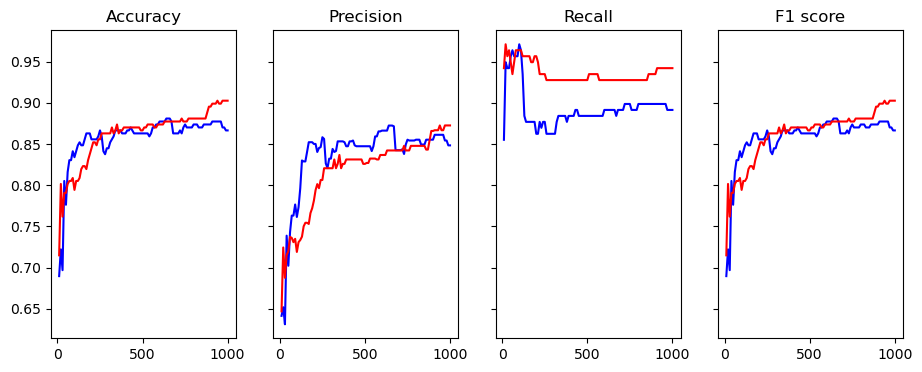
\includegraphics[width=0.8\textwidth]{images/proto_val_metrics.png}
    \caption{Accuracy, precision, recall, and f1 score on validation set. The blue plot shows the metrics for random prototype selection, the red plot for selection of prototypes with the greedy algorithm.}
    \label{fig:proto_metrics}
\end{figure*}


To obtain the final metrics on the test set, we choose the best classifier based on both the biggest difference in validation set accuracy and a minimum threshold for the accuracy of the greedy algorithm.
The accuracy of the model when using the greedy algorithm to select $S=990$ prototypes is slightly lower than random selection (79\% vs. 77\%), although this result varies depending on the initially selected random prototypes.

\begin{figure*}
    \centering
    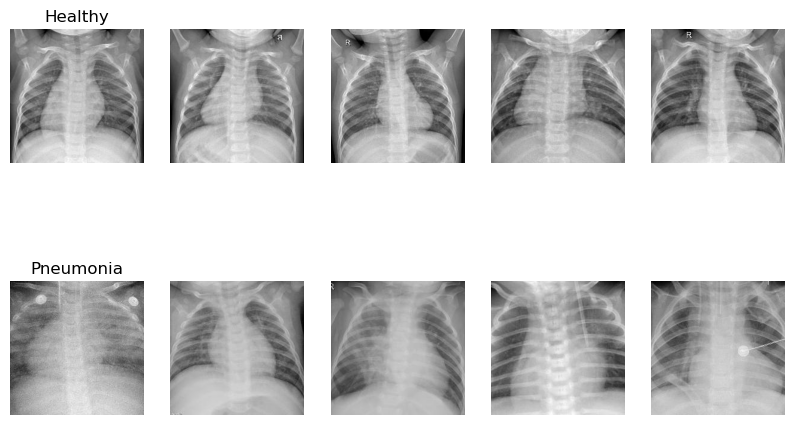
\includegraphics[width=0.8\textwidth]{images/prototypes.png}
    \caption{Prototypes of healthy (upper row) and sick (bottom row) patients, all selected by the greedy algorithm.}
    \label{fig:prototypes}
\end{figure*}

\subsection*{B. Prototype Inspection and Further Improvements}

Images from healthy patients seem relatively consistent with one another, while images from sick children vary widely (see Figure \ref{fig:prototypes}). For example, some images show clearly obfuscated lungs, while others seem to have similarly 'open' lungs, but instead thickening of the airways as the main radiological finding.

We could improve the general performance by finding criticisms, which can point to potential outliers or even mistakes in the dataset.
We could also use the output of integrated gradients, find prototypes and criticisms, and apply kNN to it.

When we compare this type of interpretable method to the previously seen saliency maps, in terms of visualization, the saliency maps provide much more information than the prototypes, simply because we see the contribution of certain features.
Of course, we can easily apply these saliency maps to the prototypes to get additional understanding on why these images might be considered good representatives of a certain class.